\section{A Synchronous Channel}

We now consider the implementation of a synchronous channel, extending the
trait in Figure~\ref{fig:SyncChanT}, using a JVM monitor.  Each
synchronisation goes through three stages, as represented in
Figure~\ref{fig:JVM-syncChan-seqDiagram}.
%
\begin{enumerate}
\item The sender  deposits its value, and signals to a receiver;

\item The receiver signals back to the sender, to provide a
  synchronisation, and returns the sender's value; 

\item The sender signals to a sender for the next synchronisation.
\end{enumerate}

%%%%%

\begin{figure}
\begin{center}
\def\height{5.2}
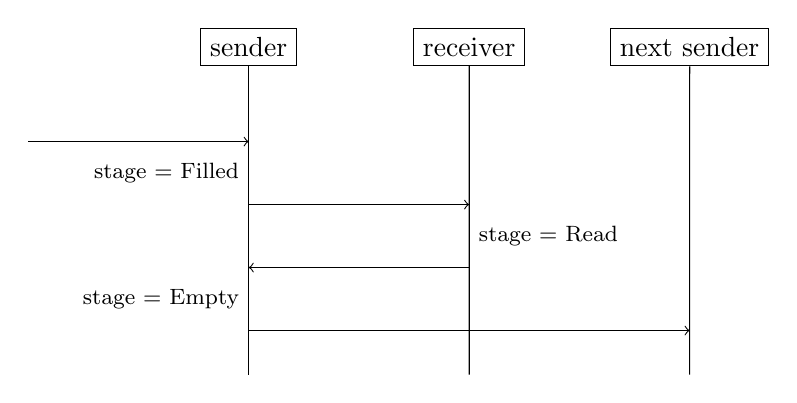
\begin{tikzpicture}[xscale = 2.8, yscale = 0.8]
\draw (0,0) node[draw] (sender) {sender};
\draw (sender) -- ++ (0,-\height);
\draw (1,0) node[draw] (receiver) {receiver}; 
\draw (receiver) -- ++ (0,-\height);
\draw (2,0) node[draw] (sender2) {next sender};
\draw (sender2) -- ++ (0,-\height);
%
\draw[<-] (sender) ++ (0,-1.5) --  ++ (-1,0); 
\draw (sender) ++ (0,-2.0) node[left]{\scalashape\footnotesize stage = Filled};
\draw[->] (sender) ++ (0,-2.5) --  ++ (1,0);
\draw (receiver) ++ (0,-3) node[right]{\scalashape\footnotesize stage = Read};
\draw[->] (receiver) ++ (0,-3.5) -- ++ (-1,0);
\draw (sender) ++ (0,-4.0) node[left]{\scalashape\footnotesize stage = Empty};
\draw[->] (sender) ++ (0,-4.5) -- ++ (2,0);
\end{tikzpicture}
\end{center}
\caption{A sequence diagram illustrating the signals in the implementation of
  a synchronous channel.}
\label{fig:JVM-syncChan-seqDiagram}
\end{figure}

%%%%%

The implementation in Figure~\ref{fig:JVM-SyncChan} uses a variable |value| to
store the sender's value, and a variable |stage| to record the current stage
of the synchronisation: whether |value| is (logically) empty, has been filled,
or whether it has been read by the receiver.

%%%%%

\begin{figure}
\begin{scala}
class JVMMonitorSyncChan[A] extends tacp.monitors.SyncChanT[A]{
  /** The current or previous value. */
  private var value = null.asInstanceOf[A]

  private val Empty = 0; private val Filled = 1; private val Read = 2

  /** The current stage of the exchange; is £value£ (logically) empty, has it been
    * filled, or has it been read by the receiver? */
  private var stage = Empty

  def send(x: A) = synchronized{
    while(stage != Empty) wait() // Wait for previous value to be consumed (1).
    value = x; stage = Filled   // Deposit my value.
    notifyAll() // Signal to receiver at (2).
    while(stage != Read) wait() // Wait for receiver (3).
    stage = Empty; notifyAll() // Signal to sender on next round at (1).
  }

  def receive(): A = synchronized{
    while(stage != Filled) wait() // Wait for sender (2).
    stage = Read; notifyAll()     // Notify current sender at (3).
    value
  }
}
\end{scala}
\caption{The implementation of a synchronous channel.}
\label{fig:JVM-SyncChan}
\end{figure}

%%%%%

Threads have to wait in three different places: the sender has to wait for the
previous synchronisation to finish; the receiver has to wait for the sender to
deposit its value; and the sender has to wait for the receiver.  As we are
using a JVM monitor, we can't target the signals to the desired place.  We
therefore have to use |notifyAll| for each signal.  Threads that receive the
signal can identify whether they should continue, or wait again, based on the
value of |stage|.

\begin{instruction}
Study the details of the implementation.
\end{instruction}
